\begin{chapter}{Introdução}

\section{Contextualização}
Grande parte das tecnologias disponíveis no mercado já estão economicamente
acessíveis para uma grande parte da população. O uso de dispositivos eletrônicos
--- como os \textit{smatphones} e os computadores pessoais --- para o auxílio de
diversas tarefas tornou-se mais recorrente no cotidiano das pessoas. Com mais
pessoas utilizando essas ferramentas está surgindo inúmeras formas de melhorar a
interação entre usuários e aparelhos eletrônicos.

Sistemas de reconhecimento ativo de gestos(AGR, do inglês \textit{actice gesture
recognition})~\cite{Darrel96}, reconhecimento automático de voz (ASR, do inglês
\textit{automatic speech recognition})~\cite{Taylor09}, síntese de voz (TTS, do inglês \textit{
text-to-speech})~\cite{Huang01}, e acionadores externos são utilizados para melhorar a 
interação humano-computador (IHC). Um sistema AGR é responsável por aplicar
técnicas de computação visual para realizar o processamento \textit{frames} de
vídeos de entrada e definir, então, na saída, qual a ação referente ao movimento
motor realizado por uma determinada parte do corpo do usuário. O ASR é o sistema
que recebe um sinal de fala digitalizado como entrada e gera um texto transcrito
na saída. O sistema TTS possui a função de gerar um sinal de voz sintetizado a
partir de um texto posto como entrada. Já os acionadores externos são
equipamentos que auxiliam as pessoas com deficiência (PCD) a utilizarem
aparelhos eletrônicos. Essas ferramentas ajudam  no controle de dispositivos
eletrônicos promovendo comodidade e praticidade às pessoas e são normalmente
enquadradas no conceito de Tecnologia Assistiva.

A Tecnologia Assistiva (TA) é uma área do conhecimento, de característica
interdisciplinar, que engloba produtos, recursos, metodologias, estratégias,
práticas e serviços que objetivam promover a funcionalidade, relacionada à
atividade e participação, de pessoas com deficiência, incapacidades ou
mobilidade reduzida, visando sua autonomia, independência, qualidade de vida e
inclusão social~\cite{cat09}.

Através da TA é possível reduzir as dificuldades vivenciadas por pessoas que
necessitam de soluções que não as deixem à margem da utilização de aparelhos
eletrônicos. Visando diminuir a exclusão digital imposta às PCD pela dificuldade
ou total incapacidade para manipular certos equipamentos, a acessibilidade é
vista como elemento fundamental para elevar a autoestima e o grau de
independência dessas pessoas.

\section{Justificativa}

Segundo dados da Organização Mundial de Saúde (WHO, do inglês \textit{World
Health Organization}), aproximadamente 15\% da população mundial possui algum
tipo de deficiência~\cite{WHO15}. Esse número é realmente expressivo, pois
revela que, em uma população de 7,6 bilhões de pessoas, cerca de um sétimo
(1~bilhão de pessoas) é portadora de deficiência. A WHO também afirma que, em
2013, 80\% das pessoas com deficiência viviam em países ainda em
desenvolvimento, o que sugere que o predomínio da condição de deficiência está
bastante relacionado com a situação econômica dos países.

No Brasil, segundo o censo realizado em 2010 pelo Instituto Brasileiro de
Geografia e Estatística (IBGE), aproximadamente 23,9\% da população (cerca de
uma entre quatro pessoas, um total de 46~milhões de habitantes) declarou ter
alguma deficiência~\cite{tIBGE}. Os dados também mostram que, desse total, quase
7\% (cerca de de 13,2~milhões) apresentam dificuldades motoras. A
Tabela~\ref{tab:ibge} mostra o perfil da população brasileira com deficiência.

\begin{table}[!h]
\centering
\caption{Perfil da população brasileira com deficiência.}
\label{tab:ibge}
\def\arraystretch{1.25}
\begin{tabular}{lccr}
	\hline
	\hline
	\textbf{Deficiência} & \textbf{Descrição} & \textbf{Número de Pessoas} &
\textbf{Porcentagem} \\
	\hline
	Visual    & Cegueira ou dificuldades gerais   & 35.774.392  & 18,754 \%  \\
	Motora    & Paralisia ou dificuldades gerais  & 13.265.599  & 6,95 \% \\
	Auditiva  & Surdez ou dificuldades gerais     & 9.717.318   &  5,094 \%  \\
	Cognitiva & Problemas mentais ou intelectuais & 2.611.536   &  1,369 \%  \\ 
	\hline
	\hline
\end{tabular}
\end{table}

Apesar da atual existência de inúmeros instrumentos voltados para Tecnologia
Assistiva como cadeiras de rodas e \textit{software} que facilitam a utilização
de computadores, grande parcela das PCD ainda não tem acesso a essas
ferramentas. A Organização Mundial de Saúde estima, por exemplo, que em países
subdesenvolvidos, aproximadamente 15\% das PCD têm acesso a essas Tecnologias
Assistivas\cite{WHO15}. Um fator que pode contribuir para esse cenário são os altos preços
de algumas dessas tecnologias. Os acionadores externos, por exemplo, apesar de
existir uma grande variedade de tipos e funcionalidades, possuem um preço bem
elevado. A Tabela~\ref{tab:acionadores} mostra os preços de alguns acionadores externos
disponíveis no mercado.

\begin{table}[!h]
\centering
\caption{Acionadores externos comerciais.}
\label{tab:acionadores}
\def\arraystretch{1.25}
\begin{tabular}{lcp{3cm}cp{3cm}}
	\hline
	\hline
	\textbf{Nome} & Ref. & \textbf{Método de acionamento} & \textbf{Comunicação} & \textbf{Custo (USD)} \\
	\hline
	Big Candy Corni&~\cite{CandyCorn}            & Aproximação  & Jack 3.5mm   & 215              \\
	Pal Pad&~\cite{PalPad}                       & Pressão      & Jack 3.5mm   &  48.75 à 61.95   \\
	Jelly Bean&~\cite{JellyBean}                 & Pressão      & Jack 3.5mm   &   65             \\
	Chin Switch&~\cite{Chin}                     & Pressão      & Jack 3.5mm   & 220              \\
	Micro Light&~\cite{MicroLight}               & Toque        & Jack 3.5mm   & 85               \\ 
	HoneyBee&~\cite{HoneyBee}                    & Aproximação  & Jack 3.5mm   & 149              \\
	AbleNet string Switch&~\cite{StringSwitch}   & Puxa corda & Jack 3.5mm & 65  \\
	Blue2 Switch&~\cite{Blue2}                   & Pressão      & Bluetooth    & 185              \\
	Savant Elite2&~\cite{SavantElite2}           & Pressão      & USB          & 38 à 181         \\
	Foot Pedal&~\cite{FootPedal}                 & Pressão      & USB          & 267              \\
	Foot Switch&~\cite{FootSwitch}               & Pressão      & USB          & 26               \\
	Sip/Puff Switch&~\cite{SipPuff}              & Sopro ou sucção & USB & 319.8  \\  
	
	\hline
	\hline
\end{tabular}
\end{table}

Acionadores que possuem como saída de comunicação o P2 Jack
como~\cite{CandyCorn}, ~\cite{PalPad}, ~\cite{JellyBean}, ~\cite{Chin}, ~\cite{
MicroLight}, ~\cite{HoneyBee} e~\cite{StringSwitch} são mais utilizados como
atuadores de um determinado circuito. Um grande exemplo disso pode ser visto no
vídeo~\cite{ATswitchYT} que mostra a ativação da fala programada de uma boneca
através do pressionamento de um acionador. Como forma de controle de uma
determinada função do computador --- como o clique de um \textit{mouse} ---
através de um acionador externo, não foi encontrado nenhum dispositivo que
utiliza a comunicação P2 Jack conectado diretamente no computador que
realiza essa tarefa. É até possível controlar o clique de um mouse com a
comunicação P2 Jack, mas é necessário o auxílio de um \textit{mouse},
como~\cite{MouseJack}, mostrado na Figura~\ref{fig:mouse}, que possua uma
adaptação que receba como entrada o P2 Jack de um acionador. Já para
acionadores como~\cite{Blue2}, ~\cite{SavantElite2}, ~\cite{FootPedal},
~\cite{FootSwitch} e ~\cite{SipPuff} que possuem comunicação Bluetooth ou USB, 
conseguem realizar o controle dos evento de
clique de \textit{mouse} facilmente sem o auxílio de outros dispositivos,
bastando apenas realizar uma pequena configuração no próprio acionador.

\begin{figure}[!h]
	\centering
	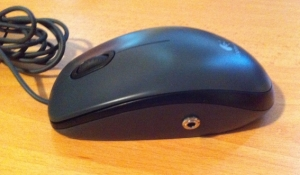
\includegraphics[width=1.0\textwidth]{fig/mouse13}
	\caption{Mouse adaptado para receber a interface P2 Jack de um acionador.}
	\label{fig:mouse}
\end{figure}

Como pode ser visto, o preço desses acionadores comerciais são bem elevados.
Algum deles possuem um mecanismo bem simples e ainda assim são vendidos a preços
absurdos. Por exemplo, o acionador~\cite{StringSwitch}, como mostrado no
vídeo~\cite{videoStringSwitch}, possui apenas uma simples corda que puxa uma
chave de fim de curso. O pino de referência é soldado no pino de refêrencia do
P2 Jack e o pino de estado da chave é soldado do pino se saída do P2 Jack.
Assim, quando o corda do acionador é puxada, os pinos de referência e saída do
P2 Jack são curto circuitados, ``simulando'' no P2 Jack os mesmos estados de
aberto e fechado da chave de fim de curso. Realizando pesquisas em sites como
MercadoLivre~\footnote{\url{https://www.mercadolivre.com.br/}}, é possível
encontrar a unidade de uma chave similar a utilizada nesse acionador custando 
cerca de R\$ 2.50. Já o pino de P2 jack custa cerca de R\$ 1. Com esses dois
materiais é possível construir um acionador semelhante ao discutido custando
menos de R\$ 10, valor bem abaixo dos U\$ 65 cobrado por esse acionador.

Na atual crise em que o Brasil se escontra, uma família de baixa renda, por
exemplo, difilcilmente iria adquidir um acionador externo devido ao elevedo
preço desses produtos, pois certamente comprometeria a renda mensal dessa
família.  Considernado que uma família possua a renda mensal de um salário
mínimo, e que esse salário está custe R\$ 954, e com o preço do dólar custando
R\$ 3.38, seria comprometido aproximadamente 23\% do salário dessa família caso
optassem por comprar esse acionador. Sendo assim, PCD de baixa renda ficam
impossibilitadas de adquirir esses produtos, excluindo-as de usufruir de
dispositivos que são voltadas para facilitar o uso de certos equipamentos que
não são adaptados para esse determinado público.

Nesse sentido, esta pesquisa tem como intuito apresentar uma solução para
diminuir a exclusão digital vivenciada pelas PCD, que muitas vezes não conseguem
utilizar aparelhos eletrônicos como \textit{smartphones} e computadores devido a
limitação de recursos que se adaptem às suas necessidades. Além disso a solução
proposta, apesar de ser voltada para o uso de uma determinada função em
aparelhos eletrônocos como computador, pode ser utilizada em outros dispositivos
que necessitem de uma interação através do pressionamento de um botão, como
ligar ou delisgar televisores e lâmpadas. O uso de acionadores externos são bons
exemplos de dispositivos que auxiliam na utilização de diversos dispositivos,
porém como grande parte dos acionadores disponíveis no mercado possuem um custo
muito elevado, há a necessidade da solução proposta ser mais acessível
economicamente para que mais PCD possam ter acesso a essas ferramentas que
auxiliam o uso de tarefas em dispositivos que normalmente não possuem interfaces
alternativas de controle. 
 
\subsection{Trabalhos Relacionados}

\textcolor{red}{Falta adicionar as revisões dos trabalhos pesquisados até que já foi feita e ta
na pasta Revisão\_Bibliografica\_tcc. Depois é só finalizar com um parágrafo
dizendo de forma breve o que vai ser proposto. Ai finaliza a parte de
justificativa}
\section{Objetivos}

\section{Síntese de Conteúdo}


\end{chapter}
